\documentclass{sysuthesis}

%%
% 论文相关信息
% 本文档中前缀"c-"代表中文版字段, 前缀"e-"代表英文版字段
% modifyer: 黄俊杰(huangjj27, 349373001dc@gmail.com)
% update date: 2017-04-13
%%

% 标题
% 论文题目应以简短、明确的词语恰当概括整个论文的核心内容,避免使用不常见的缩略词、缩写字。读者通过标题可大致了解毕业设计(论文)的内容、专业的特点和科学的范畴。中文题目一般不宜超过 24 个字,必要时可增加副标题。外文题目一般不宜超过 12 个实词

% 封面标题。由于技术所限,封面题目过长的划分交由用户您进行定夺
% 这也能让您的论文封面看起来更有美感
\covertitlefirst{中山大学}
\covertitlesecond{多维尺度问题方法与分析}

% Author:   Souler Ou
% 修改者:    欧一锋
% Date:     3/30/2018
% Mail:     ou@souler.cc
%如果英文标题过长可以使用此两项作为表三(答辩记录表)的标题。

%\etitlefirst{Unofficial \Latex\ Template}
%\etitlesecond{for SYSU Graduation Thesis}

% 另外一种封面的论文题目. 换行使用换行符("\\")
%\title{
%    中山大学 \\
%    本科毕业论文非正式模版
%}

% 中文标题
\ctitle{多维尺度问题方法与分析}
\etitle{Algorithms and analysis for methods of solving MDS problem}

% 解决英文摘要页标题过长问题 (Issue 49&63)
% 当\etitle的长度超过页边距时,请使用下面的命令自行断行
% 此操作只影响英文摘要页的标题,不影响页眉的标题
% 如果不需要断行,将\eabstracttitlesecond{ }留空即可
\eabstracttitlefirst{Algorithms and analysis for methods } 
\eabstracttitlesecond{of solving MDS problem}

% 作者详细信息
\author{熊锦欣}
\cauthor{熊\ 锦\ 欣}    % 封面作者
\eauthor{Xiong Jinxin}
\studentid{15338201}
\cschool{数学学院}

\cmajor{数学与应用数学}
\emajor{Mathematics and applied mathematics}

% 指导老师
\cmentor{李嘉\ 教授}
\ementor{Prof. Li Jia}

     % 论文相关信息
%%
% 开题报告
% modifier: 黄俊杰(huangjj27, 349373001dc@gmail.com)
% update date: 2017-05-14

% 选题目的
\objective{

}

% 思路
\methodology{

}

% 研究方法/程序/步骤
\researchProcedure{

}

% 相关支持条件
\supportment{

}

% 进度安排
\schedule{

}

% 指导老师意见
\proposalInstructions{

}

   % 开题报告内容
%%
% 摘要信息
% 本文档中前缀"c-"代表中文版字段, 前缀"e-"代表英文版字段
% 摘要内容应概括地反映出本论文的主要内容,主要说明本论文的研究目的、内容、方法、成果和结论。要突出本论文的创造性成果或新见解,不要与引言相 混淆。语言力求精练、准确,以 300—500 字为宜。
% 在摘要的下方另起一行,注明本文的关键词(3—5 个)。关键词是供检索用的主题词条,应采用能覆盖论文主要内容的通用技术词条(参照相应的技术术语 标准)。按词条的外延层次排列(外延大的排在前面)。摘要与关键词应在同一页。
% modifier: 黄俊杰(huangjj27, 349373001dc@gmail.com)
% update date: 2017-04-15
%%

\cabstract{
本文想解决的问题是当仅知道空间中$n$个点两两之间部分的距离信息时,能否有效的恢复出这$n$个点在3维空间中的坐标,并尽量保持已知的距离信息。在直接解决MDS问题的方法中,SMACOF算法可以很好的解决这种有信息缺失情况下的问题。同时受到经典多维尺度重构方法(Classical MDS,CMDS),想尽量保持已知的距离信息的要求和距离平方矩阵秩的性质的启发,本文尝试先使用低秩矩阵填充的方法恢复距离矩阵,再使用经典多维尺度重构方法,根据填充后的距离矩阵来恢复点在3维空间中的坐标。已经被证明了,当矩阵中已知的元素个数达到一定的下界时,低秩矩阵恢复问题有很大概率恢复出原来的矩阵。本文中主要介绍了SVT和OPTSPACE两种低秩矩阵恢复方法,它们可以确保在已知距离信息比例很小的情况下也能很好的恢复出相对准确的距离矩阵信息。我们给出了上述算法在$S^2$和$Cow$两个数据集上具体的数值实验过程,并展示了在不同信息缺失比例下各算法的恢复效果。对于OPTSPACE算法,分析其当数据集条件数过大时失效的原因,并提出有效的解决方法。最后进一步比较前述算法在两个数据集上的效果和差异,并分析产生差异的原因。
}
% 中文关键词(每个关键词之间用“;”分开,最后一个关键词不打标点符号。)
\ckeywords{多维尺度重构;低秩矩阵矩阵填充;SMACOF;SVT;OPTSPACE}

\eabstract{
We consider the problem of reconstructing the coordinates of $n$ points in the 3-
dimension space with only a small subset of observed entries in the distance matrix and hope
to reserve the observed information as much as possible. The SMACOF algorithm is one of
the methods for solving MDS problems that can solve the problem with missing information.
In the meantime, inspired by the classical MDS method, the requirement of reserve the observed
entries in the distance matrix and the property of the rank of squared distance matrix,
we proposed an intuitive method that is to first reconstruct the missing distance matrix using
the low-rank matrix completion algorithms and then applied classical MDS method to get the
final reconstructed coordinates in the 3-dimension space. It has been shown that when there are
enough entries in the matrix, solving the low-rank matrix completion optimization problem can
reconstruct the original matrix with high probability. In this paper, we mainly introduce two
low-rank matrix completion methods, SVT and OPTSPACE, which can efficiently reconstruct
the distance matrix even if there is only a small number of observed entries. We present the
process of the numerical test of applying the above algorithms on $S^2$ and $Cow$ dataset and show the result
of reconstructing given different sampling rate. For the OPTSPACE algorithm, we analyze
the reason for the bad performance when applied to the ill-conditioned dataset and proposed
possible efficient methods to solve it. We further compare the performance and difference of
methods proposed in this paper when applying to the two datasets and analysis the cause of such
difference.
}
% 英文文关键词(每个关键词之间用半角加空格分开, 最后一个关键词不打标点符号。)
\ekeywords{Multidimensional scaling, low-rank matrix completion, SMACOF, SVT,\\ OPTSPACE}

     % 摘要内容
%%
% 成绩评定记录表
% modifier: 黄俊杰(huangjj27, 349373001dc@gmail.com)
% update date: 2017-05-17

\gradingComment{

}
    % 成绩评定记录表评语
%%
% 四次进度报告相关信息

% Author:   Souler Ou
% 修改者:    欧一锋
% Date:     3/30/2018
% Mail:     ou@souler.cc

% 第一次进度报告
\firstsummary{
	\begin{adjustwidth}{2em}{2em}
		在这一阶段,主要完成了如下几个方面的工作:
		\begin{enumerate}
			\item 将题目范围确定在曲面重构范围内,及多位尺度变换问题,根据点与点之间的距离信息,推出一组合理的坐标。
			\item 阅读教授提供的论文,梳理基本思路,了解问题的相关背景知识与现有解决方法,基本完成论文中第一章,即引言部分的编写。
			\item 查阅与多维尺度变换方法和低秩矩阵填充方法相关的参考文献资料,并进行总结。
		\end{enumerate}
	\end{adjustwidth}
}
% 第2次进度报告
\secondsummary{
	\begin{adjustwidth}{2em}{2em}
	    在这一阶段,主要完成了如下几个方面的工作:
	    \begin{enumerate}
	        \item 完成论文中经典多维尺度变换方法和SMACOF两种方法的理论部分编写,即对应论文正文中的第二章和第三章的内容。
	        \item 对经典多维尺度变换方法和SMACOF算法在MATLAB上进行实现,并根据教授所提供的数据集和对生成坐标显示结果的函数,初步判断方法的效果,为后面的数值实验做好准备。
	    \end{enumerate}
	\end{adjustwidth}
}
% 第3次进度报告
\thirdsummary{
	\begin{adjustwidth}{2em}{2em}
		\begin{enumerate}
		    \item 确定论文后半部分方法为先用低秩矩阵填充方法恢复距离信息矩阵,再使用经典多维尺度变换方法重构出坐标。并确定论文中要涉及的低维矩阵填充方法为SVT和OPTSPACE。
		    \item 完成论文正文部分中关于SVT和OPTSPACE的理论部分编写,即对应论文正文部分的第四章和第五章。
		    \item 对SVT和OPTSPACE两种方法在MATLAB上进行实现,并在教授提供的数据集上进行基础的数值实验。
		\end{enumerate}
	\end{adjustwidth}
}
% 第4次进度报告
\fourthsummary{
	\begin{adjustwidth}{2em}{2em}
		\begin{enumerate}
		    \item 对于前面关于OPTSPACE算法的方式进行补充,添加与Incremental OPTSPACE相关的内容,并完成相应论文中内容编写和MATLAB上程序的实现。
		    \item 在之前的数值实验结果的基础上,对各个算法进行调参操作,进行记录和总结。并完成数值实验部分,即论文正文部分中的第六章的初稿。
		    \item 在教授的指导下,在数值实验章节中适当添加分析比较的部分,并将论文题目确定为“多维尺度变换问题方法与分析”。
		    \item 补充第一章引言中内容和编写中英文摘要。
		\end{enumerate}
	\end{adjustwidth}
}
% 第1次老师评价
\firstcomment{
	\begin{adjustwidth}{2em}{2em}
	\begin{enumerate}
	    \item 建议先了解多维尺度问题的定义和简单经典模型。
	    \item 尝试理解在初始信息不完整时有什么多维尺度重构的方法。
	\end{enumerate}
	\end{adjustwidth}
}
% 第2次老师评价
\secondcomment{
	\begin{adjustwidth}{2em}{2em}
		\begin{enumerate}
		    \item SMACOF是经典的解决多维尺度问题的方法,可以将其理解并实现。 
		    \item 尝试使用MATLAB对实际的曲面信息进行读取和初步处理 \item 尝试对结果进行误差分析与图示。
		\end{enumerate}
	\end{adjustwidth}
}
% 第3次老师评价
\thirdcomment{
	\begin{adjustwidth}{2em}{2em}
		\begin{enumerate}
		    \item SVT是一种简单、高效的正则化方法,值得尝试。 
		    \item OPTSPACE是指导老师未曾直接实现的方法,但因为其前沿、效果好,可以进行尝试。
		    \item 尝试对于各种方法进行分析和比较。
		\end{enumerate}
	\end{adjustwidth}
}
% 第4次老师评价
\fourthcomment{
	\begin{adjustwidth}{2em}{2em}
	    \begin{enumerate}
	        \item 首先确保各个方法具有合理的参数,基本达到理论上的最优效果。 
	        \item 应当在获取结果后,加入必要的方法原理分析和效果比较,指明好的方法为什么好。
	        \item 对于结果图示应该确保规范、整齐、减少不必要的白边。
	    \end{enumerate}
	\end{adjustwidth}
}
% 老师总评价
\finalcomment{
	\begin{adjustwidth}{2em}{2em}
		
	\end{adjustwidth}
}   % 过程检查报告数据
\begin{document}
    % 论文前置部分
    \frontmatter
        \pagenumbering{Roman}
        \maketitle    % 封面
        \makeProposal% 开题报告
        \makeProgressCheck  % 过程检查记录表
        \makeDefenseRecord  % 答辩情况等级表
        \makedisclaim       % 学术诚信声明
        \makeabstract       % 中英文摘要
        \maketableofcontents        % 目录
        \makelistoffiguretable

    % 论文主体部分
    \mainmatter
        % 引言

        % 正文
        %%
% 引言或背景
% 引言是论文正文的开端,应包括毕业论文选题的背景、目的和意义;对国内外研究现状和相关领域中已有的研究成果的简要评述;介绍本项研究工作研究设想、研究方法或实验设计、理论依据或实验基础;涉及范围和预期结果等。要求言简意赅,注意不要与摘要雷同或成为摘要的注解。
% modifier: 黄俊杰(huangjj27, 349373001dc@gmail.com)
% update date: 2017-04-15
%%

\chapter{引言}
%定义,过去的研究和现在的研究,意义,与图像分割的不同,going deeper
\label{cha:introduction}
\section{问题介绍}
多维尺度变换是一种将高维多元数据在低维空间中可视化的方法。多维尺度变换的目标是将原始数据降维到一个低维空间,并试图使低维空间中由降维产生的形变最小。一般可以将多维尺度变换解决的问题描述为:当$n$个对象之间的距离或相似性已知时,寻求这些对象在给定维数的低维空间中的表示,并使低维空间中对象间的距离与相似性与最开始给定的相似。例如,一个形象的例子:假设你有一张地图,上面有$n$个城市。通常这样的地图上会给出城市之间的距离。此时MDS所想解决的问题就是,如果只给出了城市两两之间的距离信息,能否尽可能重构出原来的地图。MDS根据涉及的对象是否可以计量分为度量型多维尺度变换(Metric MDS)和非度量型多维尺度变换(Non-metric MDS)。在度量型多维尺度变换中,又将距离度量为欧式距离的称为经典多维尺度变换(Classical MDS, CMDS)。

\section{主要内容}
本文试图解决的问题是,当已知$n$个点两两之间部分的距离信息时,能否在尽量保持距离信息的前提下,重构出三维空间中这$n$个点的坐标。显然,如果距离信息完整或者缺失比率比较少的时候,经典多维尺度变换的方法能比较有效的解决这个问题。但当距离信息缺失比例比较大的情况下,经典多维尺度变换的方法的效果就不算很好。因此,本文中介绍了一种更有效的方法,SMACOF。SMACOF试图最小化重构空间点与点之间的距离与原距离信息之间的平方误差。同时引入了一个权重变量,允许输入的给定距离信息中有缺失值,并称这个平方误差为Stress Function。最小化Stress Function的方法有很多,如Krustal\cite{kruskal1964multidimensional}的用迭代最速下降的方法来求Stress Function的最小值。Jan de Leeuw\cite{de2011applications}的SMACOF方法采用iterative majorization的方法,是一种收敛效果更好的算法。
除了上述两种经典的MDS算法之外,受经典多维尺度变换方法还有距离平方矩阵秩的性质的启发,我们考虑先通过低秩矩阵恢复的方法恢复距离矩阵信息,再使用经典多维尺度变换的方法重构出坐标。近几年解决低秩矩阵填充问题的方法有很多,如APG\cite{toh2010accelerated}(Accelerated Proximal Gradient),FPCA\cite{ma2011fixed}(Fixed Point Continuation with Approxiamte SVD),ADMIRA\cite{lee2010admira}(Atomic Decomposition for Minimum Rank Approximation)等。
本文后半部分主要介绍了两种低秩矩阵的恢复算法SVT(Singular Value Thresholding)\cite{cai2010singular}和OPTSPACE\cite{keshavan2010matrix}。尝试先使用上述两种低秩矩阵恢复的方法恢复距离信息,再使用经典多维尺度变换技术来重构坐标。最后,我们对前述算法进行数值实验,给出各算法在球面($S^2$)和牛形曲面($Cow$)两个数据集上的数值实验结果,从直观恢复结果,Error指标以及算法收敛速度三个方面来比较各算法分别在两个数据集的效果,并尝试从数据集和算法特点来分析产生效果差别的原因。

\section{本文结构与章节安排}
本文的剩余部分的结构大致如下。第 \ref{cha:classMDS}章中,我们将介绍经典多维尺度变换的背景理论和具体算法。第
\ref{cha:SMACOF}章中,我们首先介绍Majorization方法,引入Majorizing Function还有Stress Function的概念。并最后用Majorization的方法来最小化Stress function,得到最终的SMACOF算法。第 \ref{cha:SVT}章和第 \ref{cha:OPTSPACE}章中,首先介绍了距离平方矩阵秩的性质,接下来介绍SVT和OPTSPACE两种低秩矩阵恢复的方法,并在原始OPTSPACE算法的基础上引出在特殊情况下有更好效果的Incremental OPTSPACE算法。最后,在第 \ref{cha:numerical}章中,我们给出了具体的数值实验和分析过程,以及最终的分析比较的结果。
        \newclearpage
        \chapter{经典多维尺度变换}
\label{cha:classMDS}


\section{介绍}
在本小节,我们介绍一下经典多维尺度变换的基本思想。最直接的,经典多维尺度变换的想法是最小化原始距离矩阵产生的Gram矩阵和重构后的坐标产生的新的Gram矩阵之间的差。故经典多维尺度变换的想法本质上类似于PCA算法。在PCA中,“信息”用原始变量之间的总方差来表示。PCA变化之后,希望尽可能的保持变量之间的这一“信息”,即若$\mathbf{X}$表示所有的变量,$\mathbf{X}$中的每一行,记为$\mathbf{x}_i$,表示每一个单个的变量。则PCA想尽可能的保持$\sum_{i=1}^nVar(\mathbf{x}_i) = trace(\Sigma_{\mathbf{X}})$。记$\Sigma_{\mathbf{X}}$的特征值分解为$\Sigma_{\mathbf{X}} = \mathbf{U}\Lambda\mathbf{U}^\intercal$, 且$\mathbf{U}^\intercal\mathbf{U} = \mathbf{I}$。故$trace(\Sigma_{\mathbf{X}}) = trace(\Lambda) = \sum_{i=1}^n\lambda_i$,其中$\lambda_i, (i=1, \dots, n)$为$\Sigma_{\mathbf{X}}$的特征值。

由此启发,用经典多维尺度变换解决$p$维空间中的重构问题的想法是,若已知的Gram矩阵记为$\mathbf{G}$,则希望找到一个矩阵$\mathbf{G}^* = \{\mathbf{G}^*_{ij}\}$,秩为$p$,能最小化$trace(\mathbf{G} - \mathbf{G}^*) = \sum_{i=1}^n(\lambda_i - \lambda_i^*)^2$。

\section{具体算法}
我们用$\mathbf{X} = [\mathbf{x}_1, \dots, \mathbf{x}_n]^\intercal$表示点集矩阵,其中$\mathbf{X}$的一行,$\mathbf{x}_i = (x_{i1}, \dots, x_{ip})^\intercal\in\mathbb{R}^p$表示一个点的坐标,且规定$\bar{\mathbf{x}}_i = 0$。
则定义距离平方矩阵$\mathbf{D} = \{d_{ij}^2\}\in\mathbb{R}^p$,其中$d_{ij}^2 = (\mathbf{x}_i - \mathbf{x}_j)^\intercal(\mathbf{x}_i - \mathbf{x}_j)$。定义centering matrix $\mathbf{J} = \mathbf{I} - \mathbf{1}\cdot\mathbf{1}^\intercal$,其中$\mathbf{I}$为单位矩阵,$\mathbf{1}$为元素全为1的列向量。同时定义Gram matrix或称inner product matrix为$\mathbf{G = XX^\intercal}$
%%定理证明

\begin{theorem}
假设$\mathbf{J}$和$\mathbf{G}$,$\mathbf{D}$如上述定义,则有$\mathbf{G = -\frac{1}{2} JDJ}$
\end{theorem}
\begin{proof}
由定义$\mathbf{G}_{ij} = \sum_{k=1}^p x_{ik}x_{jk} = \mathbf{x}_i^\intercal \mathbf{x}_j$,$d_{ij}^2 = (\mathbf{x}_i - \mathbf{x}_j)^\intercal (\mathbf{x}_i - \mathbf{x}_j) = \mathbf{G}_{ii} + \mathbf{G}_{jj} - 2\mathbf{G}_{ij}$. 

由$\overline{\mathbf{x}}_i = 0$,则$\sum_{i=1}^n\mathbf{G}_{ij} = \sum_{j=1}^n\mathbf{G}_{ij} = 0$.

\begin{equation}
    \frac{1}{n}\sum_{i=1}^nd_{ij}^2 = \frac{1}{n}\sum_{i=1}^n\mathbf{G}_{ii} + \mathbf{G}_{jj}
\end{equation}

\begin{equation}
    \frac{1}{n}\sum_{j=1}^nd_{ij}^2 = \frac{1}{n}\sum_{j=1}^n\mathbf{G}_{jj} + \mathbf{G}_{ii}
\end{equation}

\begin{equation}
    \frac{1}{n^2}\sum_{i=1}^n\sum_{j=1}^nd_{ij}^2 = \frac{2}{n}\sum_{i=1}^n\mathbf{G}_{ii}
\end{equation}

由上述(1) (2) (3)知:
\begin{equation*}
    \mathbf{G}_{jj} = \frac{1}{n}\sum_{i=1}^nd_{ij}^2 - \frac{1}{n}\sum_{i=1}^n\mathbf{G}_{ii}
\end{equation*}

\begin{equation*}
    \mathbf{G}_{ii} = \frac{1}{n}\sum_{j=1}^nd_{ij}^2 - \frac{1}{n}\sum_{j=1}^n\mathbf{G}_{jj}
\end{equation*}

\begin{equation*}
    \frac{2}{n}\sum_{i=1}^n\mathbf{G}_{ii} = \frac{1}{n^2}\sum_{i=1}^n\sum_{j=1}^nd_{ij}^2
\end{equation*}

故带入
\begin{equation*}
    \mathbf{G}_{ij} = \frac{1}{2}(\mathbf{G}_{ii} + \mathbf{G}_{jj} - d_{ij}^2)
\end{equation*}

中得
\begin{equation*}
    \mathbf{G}_{ij} = -\frac{1}{2}(d_{ij}^2 - d_{i\cdot}^2 - d_{\cdot j}^2 + d_{\cdot\cdot}^2)
\end{equation*}
\end{proof}

%%%%第二个定理
\begin{theorem}
若$rank(\mathbf{X}) = p$,则$rank(\mathbf{G}) = rank(\mathbf{XX^\intercal}) = rank(\mathbf{X}) = p$
\end{theorem}
\begin{proof}
即要证明$\forall A\in \mathbb{R}^{n\times n}, rank(A^\intercal A) = rank(A)$。

则证明$\forall X\in \mathbb{R}^n$,$AX = 0$和$A^\intercal A = 0$同解。

首先$AX = 0$的解显然也是$A^\intercal AX = 0$的解。

另一方面由$A^\intercal AX = 0$可以推知$X^\intercal A^\intercal AX = 0$,即$(AX)^\intercal AX = 0$。故可推知$AX = 0$

故由上可知$rank(A) = rank(A^\intercal A)$,同理可知$rank(A^\intercal) = rank(AA^\intercal)$。故原等式得证。
\end{proof}

由上述两定理可知,当已知距离平方矩阵并确定重构空间维数$p$之后,我们可以得到一个秩为$p$的inner product矩阵$G$,由于矩阵$G$为对称半正定矩阵,则它应该由$p$个非零特征值和$(n-p)$个零特征值。记矩阵$G$的特征值分解为$G = U\Lambda U^\intercal$, $U_1 = (u_1, \dots, u_p)$, $\Lambda_1 = diag(\lambda_1, \dots, \lambda_p)$。则$\hat{\mathbf{X}} = U_1\Lambda_1^{\frac{1}{2}}$为重构的$p$维空间中点的坐标。具体算法见Algorithm \ref{alg: classicalMDS}。
\begin{algorithm}
\caption{经典多维尺度变换算法} 
\label{alg: classicalMDS}
\begin{algorithmic}[1]
\REQUIRE{距离矩阵$\mathbf{D}$,希望重构的空间维数$p$,点的个数$n$}
\STATE{由Theorem 1,计算$G = -\frac{1}{2}\mathbf{JDJ}$}
\STATE{计算矩阵$\mathbf{G}$的特征值分解,$G = \mathbf{U}\Lambda \mathbf{U}^\intercal$,其中$\Lambda = diag(\lambda_1,\dots,\lambda_n), \mathbf{U} = (u_1, \dots, u_n)$}
\STATE{记$\Lambda_1 = diag(\lambda_1,\dots,\lambda_p)$为$\mathbf{G}$最大的$p$个特征值,$\mathbf{U}_1 = (u_1,\dots,u_p)$为其相对应的特征向量}
\STATE{\begin{equation*}
    \mathbf{G}^* = \mathbf{U}_1\Lambda_1\mathbf{U}_1^\intercal
     = (\mathbf{U_1}\Lambda_1^{\frac{1}{2}})(\Lambda_1^{\frac{1}{2}}\mathbf{U_1})^\intercal = \mathbf{XX}^\intercal
\end{equation*}
其中$\mathbf{X} = \mathbf{U}_1\Lambda_1^{\frac{1}{2}}$}
\RETURN{$\mathbf{X}$}
\end{algorithmic}
\end{algorithm}

最后说明一下最开始假设$\bar{\mathbf{x}}_i = 0$的合理性。由$\mathbf{J\cdot1} = 0$,故$\mathbf{G\cdot1} = 0$,则
\begin{equation*}
    n^2\bar{\mathbf{X}}\bar{\mathbf{X}}^\intercal = (\bar{\mathbf{X}}^\intercal\mathbf{1})^\intercal(\bar{\mathbf{X}}^\intercal\mathbf{1}) = \mathbf{1}^\intercal\mathbf{G1} = 0
\end{equation*}
故$\bar{\mathbf{X}} = 0$。
容易发现,当距离平方矩阵完整或者缺失值较少的时候,传统MDS方法恢复的坐标效果是不错的,但是当缺失值过大之后,这种类似于主成分分析的方法是不能很好的运作的,在下一部分我们介绍一种新的MDS方法来弥补这一点。
        \newclearpage
        \chapter{SMACOF}
\label{cha:SMACOF}
\section{介绍}
不同于传统的MDS方法是想最小化恢复后的坐标产生的Gram矩阵和由已知距离矩阵生成的Gram矩阵之间的差。SMACOF方法是想直接最小化已知距离矩阵与重构的新坐标产生的距离矩阵之间的平方误差。本节中引入Stress function的定义来描述这种差值。同时在Stress function中引入一个权值,在本文中称为mask matrix。这样的操作允许输入的已知距离矩阵中有缺失值。

最小化Stress function的方法有很多,本节中将介绍Jan de Leeuw\cite{de2011applications}的一种借助iterative majorization的方法来求解Stress function的最小值的算法,即SMACOF(Scaling by majorizing a complicated function)。
\subsection{Stress Function}
与第2章中一样,定义$\mathbf{X}$为点矩阵。与前面不同,为了方便描述,此后$D$表示已观察到的距离组成的矩阵。$d_{ij}(\mathbf{X})$表示点$i$到点$j$之间的欧氏距离。则可定义mask matrix如下:

$$
W_{ij} = \left\{\begin{array}{cc}
    0 & D_{ij} = 0 \\
    1 & D_{ij} \neq 0
\end{array}\right
$$

故定义stress function:
\begin{equation}
\begin{split}
    \sigma(\mathbf{X}) &= \sum_{i<j}W_{ij}(D_{ij} - d_{ij}(\mathbf{X}))^2 = \frac{1}{2}\sum_{i,j}W_{ij}(D_{ij} - d_{ij}(\mathbf{X}))^2\\
    &= \frac{1}{2}\left(\sum_{i,j}W_{ij}D_{ij}^2 + \sum_{i,j}W_{ij}d_{ij}^2(\mathbf{X}) - 2\sum_{i,j}W_{ij}D_{ij}d_{ij}(\mathbf{X})\right)\\
    &= \frac{1}{2}\left(C + \eta^2(\mathbf{x}) - 2\rho(\mathbf{x})\right)\label{con:stressfunction}
\end{split}
\end{equation}

\section{Majorization}
这一节中将引入majorizing function和majorization的方法,然后运用此方法来求解stress function的最小值。
\begin{definition}
函数$f(x)$的majorizing function\ $g(x,z)$应满足如下三个条件:
\begin{itemize}
\item $g(x,z)$比$f(x)$更容易求最小值
\item $f(x)\leq g(x,z)$
\item $f(z) = g(z,z)$,称$z$为supporting point
\end{itemize}
\end{definition}

Majorization的主要想法是在每一次的迭代循环中,只最小化一个以Stress function为界,且与Stress function在一给定点相切的凸函数。一般情况下的Majorization最小化函数的过程如Algorithm \ref{alg: majorization}。
\begin{algorithm}
\caption{用majorization的方法求解函数$f(x)$的最小值} 
\label{alg: majorization}
\begin{algorithmic}[1]
\REQUIRE{原函数$f(x)$, majorizing function $g(x,z)$, \ep}
\STATE{Set $z = z_0$, initial value}
\WHILE{not convergent}
\STATE{计算$g(x,z)$的最小值,并记录更新的$x$值,$x^u$. 即有$g(x^u, z)\leq g(z,z)$}
\IF{$f(z) - f(x^u) < \epsilon$}
\STATE{break}
\ENDIF
\STATE{Set $z = x^u$}
\ENDWHILE
\RETURN{z}
\end{algorithmic}
\end{algorithm}

现在利用majorization的方法来求解stress function的最小值。为此,需要先找到$\sigma(\mathbf{X})$的majorization funciton。观察 (\ref{con:stressfunction})式可知,其中的第一项为一常数,接下来估计后两项$\eta^2(\mathbf{X})$和$\rho(\mathbf{X})$

首先定义矩阵$A_{ij} = \{a_{kt}\}$,

$$a_{kt} = \left\{\begin{array}{cc}
        1 & k = t = i \ \text{or}\  j  \\
        -1 & k = i, t = j \ \text{or}\  k = j, t = i \\
        0 & else
    \end{array}\right$$
记$X_k$为矩阵$\mathbf{X}$中的第$k$列,即所有点第$k$维坐标组成的列向量。注意与上一章中引入的记号$\mathbf{X}_i$表示第$i$个点的坐标向量区分开。则有:
\begin{equation*}
\begin{split}
    d_{ij}^2(\mathbf{X}) &= \sum_{k=1}^pX_k^\intercal(\mathbf{e}_i - \mathbf{e}_j)(\mathbf{e}_i - \mathbf{e}_j)^{\intercal} X_k^{\intercal}\\
    &=\sum_{k=1}^pX_k^{\intercal}A_{ij}X_k\\
    &=trace\left(\mathbf{X}A_{ij}\mathbf{X}\right)
\end{split}
\end{equation*}

则
\begin{equation*}
\begin{split}
    \eta^2(\mathbf{X}) &= \sum_{i,j}W_{ij}d_{ij}^2(\mathbf{X})
     = trace\left[\mathbf{X}\left(\sum_{i,j}W_{ij}A_{ij}\right)\mathbf{X}\right]\\
     &= trace\left(\mathbf{X}^\intercal\mathbf{V}\mathbf{X}\right)
\end{split}
\end{equation*}


其中$\mathbf{V} = \sum_{i,j}W_{ij}A_{ij} = \left\{v_{ij}\right\}$, 
$v_{ij} = \left\{\begin{array}{cc}
    -W_{ij} & i\neq j  \\
    \sum_{j=1, i\neq j}^nW_{ij} &  i = j
\end{array}\right$
\vspace{3ex}

接下来估计$\rho(\mathbf{X})$, 由Cauchy-Schwarz不等式
\begin{equation*}
    \sum_{k=1}^p(x_{ik} - x_{jk})(z_{ik} - z_{jk}) \leq\left(\sum_{k=1}^p(x_{ik} - x_{jk})^2\right)^{\frac{1}{2}} \cdot \left(\sum_{k=1}^p(z_{ik} - z_{jk})^2\right)^{\frac{1}{2}}
\end{equation*}
即
\begin{equation*}
    \sum_{k=1}^pX_k^{\intercal}A_{ij}Z_k = trace\left(\mathbf{X}^\intercal A_{ij} \mathbf{Z}\right) \leq d_{ij}(\mathbf{X}) \cdot d_{ij}(\mathbf{Z})\label{con:equal}
\end{equation*}
当且仅当$\mathbf{X = Z}$是取等。
故
\begin{equation*}
    -d_{ij}(\mathbf{X}) \leq -\frac{trace\left(\mathbf{X}^\intercal A_{ij} \mathbf{Z}\right)}{d_{ij}(\mathbf{Z})}
\end{equation*}
带入$\rho(\mathbf{X})$的表达式可得
\begin{equation}
\label{con: rho}
\begin{split}
    -\rho(\mathbf{X}) &= -\sum_{i,j}\left(W_{ij}D_{ij}\right)d_{ij}(\mathbf{X})\\
    &\leq -trace\left[\mathbf{X}^\intercal\left(\sum_{i,j}\frac{W_{ij}D_{ij}}{d_{ij}(\mathbf{Z})}\cdot A_{ij}\right)\mathbf{Z}\right]\\
    &= -trace\left(\mathbf{X}^\intercal B(\mathbf{Z})\mathbf{Z}\right)
\end{split}
\end{equation}
其中若$d_{ij}(\mathbf{Z}) = 0$,则$b_{ij} = 0$, 其余$B(\mathbf{Z}) = \{b_{ij}\}$,
$b_{ij} = \left\{\begin{array}{cc}
    -\frac{W_{ij}D_{ij}}{d_{ij}(\mathbf{Z})}   &  i\neq j \\
    -\sum_{j=1, j\neq i}^nb_{ij}     & i = j
    \end{array}\right$\\
由(\ref{con: rho})式当且仅当$\mathbf{X = Z}$时取等,则:
\begin{equation*}
    -\rho({\mathbf{X}}) \leq -trace\left(\mathbf{X}^\intercal B(\mathbf{Z}) \mathbf{X}\right) \leq -trace\left(\mathbf{X}^\intercal B(\mathbf{Z}) \mathbf{Z}\right)
\end{equation*}
若记
\begin{equation*}
    \tau(\mathbf{X,Z}) = \frac{1}{2}\left(\sum_{i,j}W_{ij}D_{ij}^2 + trace(\mathbf{X}^\intercal \mathbf{VX}) -2trace(\mathbf{X}^\intercal B(\mathbf{Z})\mathbf{Z})\right)
\end{equation*}
则可知$\sigma(\mathbf{X}) \leq \tau(\mathbf{X,Z})$, 同时可以验证majorization function中三个要求。故$\tau(\mathbf{X,Z})$可作为$\sigma(\mathbf{X})$的majorization function, 并且为关于变量$\mathbf{X}$的二次函数。故最小值可以通过令导数为零来求解。即求解$\nabla_{\tau}(\mathbf{X,Z}) = \mathbf{VX}- B(\mathbf{Z})\mathbf{Z} = 0$。由于$\mathbf{V}$不一定满秩,故用Moore-Penrose inverse来进行求解,记广义逆为$\mathbf{V}^+ = (\mathbf{V} + \mathbf{11}^\intercal)^{-1} - n^{-2}\mathbf{11}^\intercal$,则$\mathbf{X}^u = \mathbf{V}^+B(\mathbf{Z})\mathbf{Z}$。

至此我们找到了stress function的majorization function并且知道了其算法的更新规则。结合Algorithm \ref{alg: majorization}中的结论,可以得到最终的SMACOF算法。

%%%%%%%%具体算法

\section{SMACOF算法}
\begin{algorithm}
\caption{SMACOF算法} 
\label{alg: SMACOF}
\begin{algorithmic}[1]
\REQUIRE{随机初始值$\mathbf{X}$,$\mathbf{Z = X}$, $\epsilon = 10^{-4}$, $k=0$, MaxIter = 1000}
\STATE Set sigma = $\sigma(\mathbf{X})$, sigma\_old = sigma
\WHILE {$k=0$ \ \text{or} \ (sigma\_old - sigma > $\epsilon$ \ \text{and}\ k $\leq$ MaxIter)}
\STATE{sigma\_old = sigma}
\STATE{$k = k + 1$}
\STATE{$\mathbf{X} = \mathbf{V}^+B(\mathbf{Z})\mathbf{Z}$}
\STATE{sigma = $\sigma(\mathbf{X})$}
\STATE{$\mathbf{Z = X}$}
\ENDWHILE
\RETURN{$\mathbf{Z}$}
\end{algorithmic}
\end{algorithm}
至此我们介绍了两种直接利用已有的距离矩阵来恢复坐标的方法。由数值计算结果可知,SMACOF即使是在距离矩阵缺失较为严重的时候也能很好的恢复出坐标。受经典MDS方法的启发,接下来,本文将介绍两种低秩矩阵填充方法。尝试先恢复距离矩阵,之后再使用经典MDS方法来恢复坐标。

        \newclearpage
        \chapter{SVT}
\label{cha:SVT}
\section{介绍}
接下来我们所需要解决的问题可描述为:根据一小部分已知的元素,重构或者恢复一个$n\times n$低秩矩阵$\mathbf{M}$。精确矩阵填充问题(exact matrix completion problem)等价于找到一个秩最小的矩阵与已知的矩阵元素相对应。即:
\begin{align}
\label{al: rank}
&\min \ rank(\mathbf{X}) \nonumber\\
s.t.\ &\mathbf{X}_{ij} = \mathbf{M}_{ij}, (i,j)\in \Omega
\end{align}
这是一个NP-Hard问题,在压缩感知(compressed sensing)领域中,一个核心的问题就是找到满足一系列限制条件的最稀疏的向量。即:
\begin{align*}
&\min \ \left\|x\right\|_{l_0}\\
s.t.\ &Ax = b,
\end{align*}
其中$l_0$范数表示向量的稀疏性,即向量中非零元素的个数。为了解决这个问题,一个通用的方法是解决下面的优化问题:
\begin{align*}
&\min \ \left\|x\right\|_{l_1}\\
s.t.\ & Ax = b,
\end{align*}
其中$l_1$范数是向量中所有元素绝对值之和。$l_1$范数的优化问题,在适当的条件下可以提供原$l_0$问题的最优解。现在回到原来的优化问题(\ref{al: rank}),秩可以视为矩阵非零奇异值的个数,而核范数是矩阵所有奇异值之和。故可以将矩阵$rank(\cdot)$类比成向量的$l_0$范数,矩阵的核范数$\|\cdot\|_*$可以对应成$l_1$范数。矩阵秩的优化问题和压缩感知问题之间的联系在\cite{recht2010guaranteed}中有详细的研究。由上述想法Candes and Recht将(\ref{al: rank})中的问题凸松弛化为核范数的优化问题,即最小化奇异值的和\cite{candes2009exact}。如下:
\begin{align}
\label{al:optimize}
&\min \ \left\|\mathbf{X}\right\|_* , \nonumber\\
s.t.\ &\mathbf{X}_{ij} = \mathbf{M}_{ij}, (i,j)\in \Omega
\end{align}
同时\cite{candes2009exact}中证明了,对于一个$m\times n$秩为$r$的矩阵$\mathbf{M}$,当已知元素个数$|\Omega|$满足,$|\Omega|\geq C(\alpha) r n^{1.2}log(n)$,且满足incoherence的性质时,解决问题(\ref{al:optimize})可以很大概率的恢复矩阵$\mathbf{M}$。

SVT就为解决问题(\ref{al:optimize})的方法之一。 同时相较于\cite{liu2009interior}中的interior point方法, SVT更能解决数据量比较大的情况下的问题。SVT算法是一种迭代算法,产生一个矩阵序列$\{\mathbf{X}^k,\mathbf{Y}^k\}$。每一步的迭代操作主要就是对矩阵$\mathbf{Y}^k$的奇异值进行一个软阈值操作(soft-thresholding operation)。由于$\mathbf{Y}^k$为一稀疏矩阵,SVT算法有每一次迭代中计算代价低,存储空间要求低的优点。


\section{距离平方矩阵的低秩性}
与前面的定义相同,$\mathbf{X} = [\mathbf{x}_1, \dots, \mathbf{x}_n]$, $\mathbf{x}_i \in \mathbb{R}^p$,并假设$p\ll n$,$\mathbf{D}$为距离平方矩阵。\cite{dokmanic2015euclidean}中提出了距离平方矩阵的秩应满足的性质,我们将它叙述成定理并给出相应证明如下:
\begin{theorem}
$rank(\mathbf{D}) \leq (p+2)$
\end{theorem}

\begin{proof}
由
\begin{equation*}
    D = \mathbf{1} \cdot diag(\mathbf{X}^\intercal\mathbf{X})^\intercal + diag(\mathbf{X}^\intercal\mathbf{X}) \cdot \mathbf{1}^\intercal - 2 \mathbf{X}^\intercal\mathbf{X}
\end{equation*}

由$rank(\mathbf{X})\leq p$, 则$rank(\mathbf{X}^\intercal\mathbf{X}) \leq p$。又上式中的其他两项的秩均为$1$,由秩的性质知
\begin{equation*}
\begin{split}
    rank(\mathbf{D}) &\leq rank(\mathbf{1} \cdot diag(\mathbf{X}^\intercal \mathbf{X})) + rank(diag(\mathbf{X}^\intercal\mathbf{X}) \cdot \mathbf{1}^\intercal) - rank(2\mathbf{X}^\intercal\mathbf{X})\\
    &\leq p + 2
\end{split}
\end{equation*}
\end{proof}
故由上定理可知距离平方矩阵的秩最大只能为$(p + 2)$,故当$d\ll n$时,$rank(\mathbf{D})\ll n$。故接下来试图采用低秩矩阵的恢复方法来恢复距离平方矩阵。

\section{SVT算法}
在本小节将介绍\cite{cai2010singular}中的SVT算法来解决(\ref{al:optimize})中的优化问题,首先定义一个正交算子$P_{\Omega}$
$$
P_{\Omega}(\mathbf{M})_{ij} = \left\{\begin{array}{cc}
     \mathbf{M}_{ij} & (i,j) \in\Omega \\
     0 & otherwise
\end{array}
$$
故优化问题可写成
\begin{align}
\label{al: ortho}
&\min \ \left\|\mathbf{X}\right\|_*\nonumber\\
s.t.\ & P_{\Omega}(\mathbf{M}) = P_{\Omega}(\mathbf{X})
\end{align}
依照\cite{cai2010singular}中,对于给定的软阈值$\tau$和步长序列$\{\delta_k\}$,初值$\mathbf{Y}_0$,有迭代算法:
$$
\left\{\begin{array}{cc}
\label{arr: iter}
     \mathbf{X}^k &= \mathbf{D}_\tau(\mathbf{Y}^{k-1}) \nonumber\\
     \mathbf{Y}^k &= \mathbf{Y}^{k-1} + \delta_kP_\Omega(\mathbf{M} - \mathbf{X}^k)
\end{array}\right
$$
其中$D_{\tau}$为Shrinkage operator。若$\mathbf{X}\in\mathbb{R}^{n_1\times n_2}, rank(\mathbf{X}) = r$,记$\mathbf{X}$的奇异值分解为$\mathbf{X = U}\Sigma \mathbf{V}^\intercal, \Sigma = diag\left(\{\sigma_i\}_{1\leq i \leq r}\right), \mathbf{U}\in\mathbb{R}^{n_1\times r}, \mathbf{V}\in \mathbb{R}^{n_2\times r}$
则
\begin{equation*}
\mathbf{D}_\tau(\mathbf{X}) = \mathbf{U}\mathbf{D}_\tau(\Sigma)\mathbf{V}^\intercal, 
\mathbf{D}_\tau(\Sigma) = diag(\{\sigma_i - \tau\}_+)
\end{equation*}

在\cite{cai2010singular}中已经证明$\{ \mathbf{X}^k\}$序列收敛到如下优化问题的解
\begin{align*}
&\min \ \tau\left\|\mathbf{X}\right\|_* + \frac{1}{2}\left\|\mathbf{X}\right\|_F^2  \\
s.t.\ & P_{\Omega}(\mathbf{M}) = P_{\Omega}(\mathbf{X})
\end{align*}
而当$\tau \to \inf$时,上述优化问题即逼近(\ref{al: ortho})式的解。
由\cite{cai2010singular}中已经证明,当步长$\delta$大于0,小于2时的时候,该算法一定收敛,但是收敛速度会很慢。故采用论文中建议的数值,即若$|\Omega|=m$,则$\delta = 1.2\frac{n_1n_2}{m}$。

关于$\mathbf{Y}^0$初值的选择,记$k_0$为满足如下条件的整数
\begin{equation*}
    \frac{\tau}{\delta\|P_\Omega(\mathbf{M})\|_2}\in (k_0-1, k_0].
\end{equation*}
由于$\mathbf{Y}^0 = \mathbf{0}$,根据前面的迭代算法可以看出,$\mathbf{X}^k = \mathbf{0}$且$\mathbf{Y}^k = k\delta P_{\Omega}(\mathbf{M})$,$k = 1,\dots,k_0$。故可以跳过计算$\mathbf{X}^1,\dots,\mathbf{X}^{k_0}$的过程,直接以$Y^0 = k_0\delta P_\Omega(\mathbf{M})$为初值开始。最后关于迭代的终止条件,\cite{cai2010singular}中给出的SVT算法的迭代终止条件为
\begin{equation*}
    \frac{\|P_{\Omega}(\mathbf{X}^k - \mathbf{M})\|_F}{\|P_{\Omega}(\mathbf{M})\|_F} \leq \epsilon
\end{equation*}
下面给出$\mathbf{M}\in \mathbb{R}^{n\times n}$情形下的算法。

\begin{algorithm}
\caption{SVT算法} 
\label{alg3}
\begin{algorithmic}[1]
\REQUIRE{$l = 5, \delta = 1.2\frac{n^2}{|\Omega|}, k_0 = \text{ceil}(\frac{\tau}{\delta\left\|P_\Omega(\mathbf{M})\right\|_2})$, $r_0 = 0, \mathbf{Y}^0 = k_0\delta P_\Omega(\mathbf{M})$, MaxIter = 1000, $tol = 1^{-4}$}
\FOR{k = 1: MaxIter}
\STATE{set $S_k = \min(r_{k-1} + l, n)$}
\REPEAT
\STATE{[$\mathbf{U}^{k-1}, \Sigma^{k-1}, \mathbf{V}^{k-1}]_{s_k} = svds(\mathbf{Y}^{k-1}, s_k)$}
\STATE{Set $s_k = \min(s_k + l,n)$}
\UNTIL{$\sigma_{s_{k-l}}^{k-1} \leq \tau$}
\STATE{$r_k = max\{j: \sigma_j^{k-1} > \tau\}$}
\STATE{$\mathbf{X}^k = \sum_{j=1}^{r_k}(\sigma_j^{k-1} - \tau)u_j^{k-1}v_j^{k-1}$}
\IF{$\frac{\left\|P_\Omega(\mathbf{X}^k - \mathbf{M})\right\|_F}{\left\|P_\Omega(\mathbf{M})\right\|_F} \leq tol$}
\STATE{break}
\ENDIF
\STATE{Set $$\mathbf{Y}_{ij}^k = \left\{\begin{array}{cc}
    \mathbf{Y}_{ij}^{k-1} + \delta(\mathbf{M}_{ij} - \mathbf{X}_{ij}^k) & (i,j) \in \Omega \\
   0 & (i,j) \notin \Omega
\end{array}\right$$}
\ENDFOR
\RETURN{$\mathbf{X}^k$}
\end{algorithmic}
\end{algorithm}
        \newclearpage
        \chapter{OPTSPACE}
\label{cha:OPTSPACE}
\section{介绍}
OPTSPACE是\cite{keshavan2009gradient}中提出的基于奇异值分解的解决低秩矩阵填充的方法。由上章知,\cite{candes2009exact}提出了对于精确矩阵填充的已知元素的下界$|\Omega|\geq C(\alpha)rn^{1.2}log(n)$,而\cite{keshavan2010matrix}将此下界推进到$|\Omega| \geq C(\alpha)rn\max \{log(n), r\}$。
算法的想法是去最小化cost function。记
$$\mathbf{M}_\Omega = \left\{\begin{array}{cc}
    \mathbf{M}_{ij} & (i,j) \in \Omega \\
    0 & (i,j) \notin \Omega 
\end{array}\right$$ 
$rank(\mathbf{M}) = r$, 则可以定义cost function,$F:\mathbb{R}^{n\times r} \times \mathbb{R}^{n \times r} \to \mathbb{R}$如下:
\begin{equation*}
    \mathcal{F}(\mathbf{X}, \mathbf{Y}, S) = \frac{1}{2}\sum_{(i,j)\in\Omega}\left[\mathbf{M}_{ij} - (\mathbf{X}S\mathbf{Y}^\intercal)_{ij}\right]^2
\end{equation*}
\begin{equation*}
    F(\mathbf{X,Y}) = \min_{S\in\mathbb{R}^{r\times r}}\mathcal{F}(\mathbf{X,Y},S)
\end{equation*}
其中$\mathbf{X}\in\mathbb{R}^{n\times r}, \mathbf{Y}\in\mathbb{R}^{n\times r}$, 且$\mathbf{X}^\intercal\mathbf{X} = \mathbf{Y}^\intercal\mathbf{Y} = n\mathbf{I}$。
至此我们可以考虑用梯度下降法来求解cost function的最小值,而$\mathbf{M}_\Omega$的奇异值分解,可以作为梯度下降法的初值猜测。接下来先介绍一些算法中的定义,最后再给出完整的算法。
\section{Trimming}
\label{con: trim}
Trimming的操作是删去矩阵中过度表达的行与列,即degree超过$\frac{2|\Omega|}{n}$的行与列全部重置为0,用$d_c(i), d_r(i)$表示矩阵中的第i列和第j列的degree,故Trimming即
$$
    Tr(\mathbf{M}_\Omega) = \left\{\begin{array}{cc}
        0 & d_c(i) > \frac{2|\Omega|}{n} \ \text{or}\ d_r(j) > \frac{2|\Omega|}{n} \\
        (\mathbf{M}_\Omega)_{ij} & otherwise 
    \end{array}\right
$$
Trimming的操作有一点违反我们的思维,因为这一步我们似乎丢掉了一些有用的信息。但这样做是很重要的。当n比较大的时候,对于矩阵的奇异值分解后的奇异值将集中在这些过度表达的行或列,而不能表是足够的缺实值的信息。通过Trimming的操作可以有效的防止这一问题。

\section{Rank-p projection}
Rank-p projection可以视作是对$Tr(\mathbf{M}_\Omega)$进行奇异值分解,并对得到的奇异值和奇异向量进行尺度变换。即得到$Tr(\mathbf{M}_\Omega) = \sum_{i=1}^nx_i\sigma_iy_i^\intercal$。故可定义Rank-p projection为
$\mathcal{P}_p$: 
\begin{equation*}
    \mathcal{P}_p(Tr(\mathbf{M}_\Omega)) = \mathbf{X}_0S_0\mathbf{Y}_0^\intercal
\end{equation*}
其中$\mathbf{X}_0\in\mathbb{R}^{n \times p}, \mathbf{Y}_0\in\mathbb{R}^{n\times p}$, $S_0$为$p\times p$的对角矩阵,
分别定义为$\mathbf{X}_0 = \sqrt{n}(x_1,\dots,x_p), \mathbf{Y}_0 = \sqrt{n}(y_1,\dots,y_p), S_0 = \frac{n}{|\Omega|}diag(\sigma_1,\dots,\sigma_p)$

\section{Gradient descent}
为了方便后面的描述,记$\overrightarrow{x} = (\mathbf{X,Y})$将$\mathcal{F}$改写如下:
\begin{equation*}
    \mathcal{F}(\mathbf{X,Y},S) = \frac{1}{2}\left\|P_{\Omega}(\mathbf{M} - \mathbf{X}S\mathbf{Y}^\intercal)\right\|_F^2
\end{equation*}
则
\begin{equation*}
    gradF(\overrightarrow{x})_{\mathbf{X}} = P_\Omega(\mathbf{X}S\mathbf{Y}^\intercal - \mathbf{M})\mathbf{Y}S^\intercal
\end{equation*}
\begin{equation*}
    gradF(\overrightarrow{x})_{\mathbf{Y}} = P_\Omega(\mathbf{X}S\mathbf{Y}^\intercal - \mathbf{M})^\intercal\mathbf{X}S
\end{equation*}
故$gradF(\overrightarrow{x_k}) = (gradF(\overrightarrow{x_k})_{\mathbf{X}},gradF(\overrightarrow{x_k})_{\mathbf{Y}})$,则由初值$\overrightarrow{x_0} = (\mathbf{X}_0,\mathbf{Y}_0)$, 可以进行梯度下降来求解最小值。\cite{armijo1966minimization}中证明了对于任意大小的$\tau$,OPTSPACE算法都可以收敛到局部最小值,并指出$\tau = 10^{-3}$为一个在实际应用中较好的选择。最后关于OPTSPACE算法的终止条件,与上一节中SVT算法的终止条件相同,即$\|P_{\Omega}(\mathbf{X} - \mathbf{M})\|_F/\|P_{\Omega}(\mathbf{M})\|_F \leq tol$。综上,完整的OPTSPACE算法可以叙述如下:

\section{OPTSPACE算法}
\begin{algorithm}
\caption{OPTSPACE算法} 
\label{alg4}
\begin{algorithmic}[1]
\REQUIRE{$\mathbf{M}_\Omega$, step size\ $\tau = 10^{-3}$, MaxIter = 1000, tol = $10^{-4}$, rank $r$}
\STATE{Trim $\mathbf{M}_\Omega \Rightarrow \ Tr(\mathbf{M}_\Omega)$}
\STATE{$\mathcal{P}_r(\mathbf{M}_\Omega) = \mathbf{X}_0S_0\mathbf{Y}_0^\intercal$ $\Rightarrow \overrightarrow{x_0} = (\mathbf{X}_0, \mathbf{Y}_0)$}
\FOR{$k = 0, \dots, $MaxIter}
\STATE{$s_k = \arg \min_S \mathcal{F}(\mathbf{X}_k, \mathbf{Y}_k, S)$}
\STATE{$\overrightarrow{w_k} = gradF(\overrightarrow{x_k})$}
\STATE{Set $t_k = \tau$}
\WHILE{$F(\overrightarrow{x_k}-t_k\overrightarrow{w_k}) - F(\overrightarrow{x_k}) > \frac{1}{2}t_k\left\|\overrightarrow{w_k}\right\|^2$}
\STATE{$t_k = \frac{t_k}{2}$}
\ENDWHILE
\STATE{Set $\overrightarrow{x_{k+1}} = \overrightarrow{x_k} - t_k\overrightarrow{w_k}$}
\IF{$\frac{\left\|P_\Omega(\mathbf{M} - \hat{\mathbf{M}})\right\|_F}{\left\|P_\Omega(\mathbf{M})\right\|_F} < tol$}
\STATE{break}
\ENDIF
\ENDFOR
\RETURN{$\Hat{\mathbf{M}} = \mathbf{X}_kS_k\mathbf{Y}_k^\intercal$}
\end{algorithmic}
\end{algorithm}

关于第4步中求解$S$的方法,由于$\mathcal{F}$为关于$S$的二次函数,故求导等于0来求解。
\begin{equation*}
\begin{split}
    \frac{d\mathcal{F}(\mathbf{X,Y},S)}{dS_{ij}} &= \frac{1}{2}P_\Omega\frac{d<\mathbf{M}_\Omega - \mathbf{X}S\mathbf{Y}^\intercal, \mathbf{M}_\Omega - \mathbf{X}S\mathbf{Y}^\intercal>_{ij}}{dS_{ij}}\\
    &=-\frac{1}{2}P_\Omega\frac{<\mathbf{M}_\Omega - \mathbf{X}S\mathbf{Y}^\intercal, d\mathbf{X}S\mathbf{Y}^\intercal>_{ij}}{dS_{ij}}\\
    &=-\frac{1}{2}P_\Omega\frac{<\mathbf{X}^\intercal(\mathbf{M}_\Omega - \mathbf{X}S\mathbf{Y}^\intercal)_{ij}\mathbf{Y}, dS>}{dS_{ij}} = 0
\end{split}
\end{equation*}
故可以得到
\begin{equation*}
    \left[\mathbf{X}^\intercal(\mathbf{X}_{\cdot i}\mathbf{Y}_{\cdot j}^\intercal)\mathbf{Y}\right]S_{ij} = \mathbf{X}^\intercal(\mathbf{M}_\Omega)_{ij}\mathbf{Y}
\end{equation*}
可以求解出矩阵$S$。

同时注意,OPTSPACE算法中需要提前给出恢复矩阵的秩,
\cite{keshavan2009gradient}中给出了一种估计稀疏矩阵秩的方法。记$\epsilon = |\Omega|/n$,同时如第\ref{con: trim}节中对Trimming操作之后的矩阵进行奇异值分解即:
\begin{equation*}
    Tr(\mathbf{M}_{\Omega}) = \sum_{i=1}^n x_i\sigma_iy_i^\intercal
\end{equation*}
则基于奇异值可以定义如下的损失函数:
\begin{equation*}
    R(i) = \frac{\sigma_{i+1} + \sigma_i\sqrt{\frac{i}{\epsilon}}}{\sigma_i}
\end{equation*}
则可估计填充后的矩阵$\mathbf{M}$的秩为使$R(i)$取最小值的下标$i$。这个算法之后的想法是,如果$|\Omega|$足够大,则当把奇异值按从大到小排列的时候,会发现第$r+1$个和第$r$个奇异值之间的差很大。故可以预测完整的$\mathbf{M}$矩阵的秩为$r$。但当$|\Omega|$相对较小或者矩阵的条件数较大的时候,这个算法的结果和真实值的误差就很大。但由距离平方矩阵秩的性质,我们希望在三维空间中重构坐标,则距离平方矩阵的秩最大不会超过5。我们不妨尝试所有可能的秩的值,分别带入算法,最后选取效果相对好小的最小的秩作为最终带入算法中进行恢复的参数。

\section{Incremental OPTSPACE}
原始的OPTSPACE算法有一个缺陷,就是当带入算法的数据矩阵的条件数太大的时候,OPTSPACE算法无法很好的考虑到较小的奇异值的贡献。其中条件数定义为$k = \frac{\sigma_1(\mathbf{M})}{\sigma_r(\mathbf{M})}$,$r$为矩阵$\mathbf{M}$的秩,$\sigma_i(\mathbf{M})$表示矩阵$\mathbf{M}$从大到小排序第$i$个奇异值。即当以原始矩阵奇异值分解作为初始值带入梯度下降算法中时,会落入一个局部最小值,并只展现出相对较大的几个特征值所产生的结构特征,而忽略较小奇异值产生的影响。在第
\ref{cha:numerical}章中对于$Cow$数据集的实验中我们就可以看到这一缺陷。为解决条件数较大情形下的问题,\cite{keshavan2009gradient}中提供了一种名为Incremental OPTSPACE的算法。其主要的想法是每次迭代中,只计算最大的奇异值所产生的贡献,并在下一次迭代中删去这一部分贡献。这样做可以保证那些较小的奇异值也被充分的应用,进而达到相对原始OPTSPACE算法更好的效果。具体算法如下:

\begin{algorithm}
\caption{Incremental OPTSPACE算法} 
\label{alg6}
\begin{algorithmic}[1]
\REQUIRE{$\mathbf{M}_\Omega$, step size\ $\tau = 10^{-3}$, MaxIter = 500, tol = $10^{-4}$, rank $r$}
\STATE{Trim $\mathbf{M}_\Omega \Rightarrow \ Tr(\mathbf{M}_\Omega)$}
\STATE{Set $\Hat{\mathbf{M}} = 0$}

\FOR{$k = 0, \dots, r$}
\STATE{计算$\mathbf{M}_\Omega - \Hat{\mathbf{M}}$最大的奇异向量$(u, v)$}
\IF{$k = 0$}
\STATE{$\mathbf{X}_0 = u; \mathbf{Y}_0 = v$}
\ELSE
\STATE{$\mathbf{X}_0 = [\mathbf{X}, u]; \mathbf{Y} = [\mathbf{Y}, v]$}
\ENDIF
\STATE{$\overrightarrow{x_0} = (\mathbf{X}_0, \mathbf{Y}_0)$}

\FOR{$k = 0, \dots, $MaxIter}
\STATE{$s_k = \arg \min_S \mathcal{F}(\mathbf{X}_k, \mathbf{Y}_k, S)$}
\STATE{$\overrightarrow{w_k} = gradF(\overrightarrow{x_k})$}
\STATE{Set $t_k = \tau$}
\WHILE{$F(\overrightarrow{x_k}-t_k\overrightarrow{w_k}) - F(\overrightarrow{x_k}) > \frac{1}{2}t_k\left\|\overrightarrow{w_k}\right\|^2$}
\STATE{$t_k = \frac{t_k}{2}$}
\ENDWHILE
\STATE{Set $\overrightarrow{x_{k+1}} = \overrightarrow{x_k} - t_k\overrightarrow{w_k}$}
\IF{$|\mathbf{F}(x_{k+1}) - \mathbf{F}(x_k)| \leq tol\mathbf{F}(x_k)$}
\STATE{break}
\ENDIF
\STATE{$\Hat{\mathbf{M}} = \mathbf{X}_kS_k\mathbf{Y}_k$}
\ENDFOR
\ENDFOR
\RETURN{$\Hat{\mathbf{M}}$}
\end{algorithmic}
\end{algorithm}

        \newclearpage
        \chapter{数值实验}
\label{cha:numerical}
本章中主要对两个数据集来进行实验。一个取样于一个单位球面($S^2$),包含$1002$个点,另一个取样于一个牛形的曲面($Cow$),包含$2602$个点。本节中首先比较不同sampling rate下前述算法重构距离矩阵的相对误差,即
\begin{equation*}
    \text{Error} = \frac{\|\mathbf{X}-\mathbf{M}\|_F}{\|\mathbf{M}\|_F}
\end{equation*}
其中,由于数据是从点集中随机取样,故表格中用5次实验的误差的均值来进行比较。同时算法中的一些需要预先确定的参数,在没有特殊说明的情况下,参见前面各算法表述中   \textbf{Require}。

本节的实验主要分为三个部分,第一部分首先确认两个数据集所要带入OPTSPACE算法中的秩的大小。第二部分展示SMACOF, 和基于SVT还有OPTSPACE和经典多维尺度变换的算法,在处理不同sampling rate下两个数据集的结果。并对于数值实验的结果进行分析总结。最后一部分,我们分析比较各算法在两个数据集上的表现与效果,并分析产生差异的原因。


首先,先来判断两个数据集的秩。分别对两个数据集在sampling rate比较大的情况下分别用不同的秩带入算法,通过比较Error的情况来确定所要带入算法中的秩的大小。为此,本文中先针对sampling rate分别为$30\%, 50\%$和$70\%$的情况,将$rank = 1, 2, 3, 4, 5$分别带入参数为$tau = 10^{-3}$的OPTSPACE算法,然后选取使Error相对较小的秩中最小的一个。
\begin{table}[!htbp]
\centering
\begin{tabular}{|c|ccccc|}
\hline
\diagbox{rate}{Error}{rank}&1 &2 &3 &4 &5\\
\hline
\text{30\%}&0.3375 &0.2278 &0.1982 &1.094E-4 &1.095E-5 \\
\hline
\text{50\%}&0.3372 &0.2773 &0.1977 &9.758E-5 &9.887E-5\\
\hline
\text{70\%}&0.3370 &0.2770 &0.1974 &6.300E-5 &6.351E-5\\
\hline
\end{tabular}
\caption{$S^2$数据集sampling rate为30\%,50\%和70\%情况下秩为1\~{}5分别带入OPTSPACE算法作为参数的Error}
\label{tab: sphere_rank}
\end{table}

\begin{table}[!htbp]
\centering
\begin{tabular}{|c|ccccc|}
\hline
\diagbox{rate}{Error}{rank}&1 &2 &3 &4 &5\\
\hline
\text{30\%}&0.4586 &0.1411 &0.0686 &0.0686 &0.0686 \\
\hline
\text{50\%}&0.4583 &0.1411 &0.0685 &0.0428 &0.0428\\
\hline
\text{70\%}&0.4584 &0.1410 &0.0685 &0.0412 &0.0159\\
\hline
\end{tabular}
\caption{$Cow$数据集sampling rate为30\%,50\%和70\%情况下秩为1\~{}5分别带入OPTSPACE算法作为参数的Error}
\label{tab: cow_rank}
\end{table}

由表\ref{tab: sphere_rank}和表\ref{tab: cow_rank}可见,对于$S^2$中各个sampling rate,Error都是在秩为$4$的带入算法的时候最小。对于$Cow$数据集中当sampling rate为$70\%$时,当秩为$5$的时候Error才达到最小。故$S^2$数据集应带入$rank = 4$,$Cow$数据集中应带入$rank = 5$。同时从表\ref{tab: cow_rank}中可以看见当sampling rate为$30\%$时,从$rank = 3$开始,Error已经不再发生变化,并观察到在$30\%, 50\%, 70\%$这样较大的sampling rate下,$Cow$数据集中的Error仍然很大。由此可以预估$Cow$数据集可能存在条件数比较大的情况,并进而影响了OPTSPACE算法在该数据集上的效果。在后面的实验中也验证了我们这一猜测。



%\begin{figure}
%\centering 
%\includegraphics[totalheight=4.8in]{SpherePlot.png} 
%\caption{不同sampling rate下$S^2$三种算法恢复结果图} 
%\label{fig:sphere} 
%\end{figure}
\begin{figure}[h]
	\centering
	\includegraphics[width=1.0\textwidth]{figure/SpherePlot.png}
	\caption{不同sampling rate下三种算法恢复$S^2$数据集结果图}
 	\label{fig:sphere}
\end{figure}

\begin{table}[!htbp]
\caption{不同Sampling Rate下不同算法重构的$S^2$距离矩阵的误差}
\label{tab: sphere}
\centering
\begin{tabular}{|c|ccccc|}
\hline
\diagbox{Algorithm}{Error}{Sampling rate}&$2\%$ &$3\%$ &$5\%$ &$10\%$ &$20\%$\\
\hline
\text{SMACOF}&0.0200 &2.070E-4 &1.162E-4 &4.7375E-4 &2.9069E-5 \\
\hline
\text{SVT+CMDS}&0.1889 &1.731E-4 &1.753E-4 &1.450E-4 &1.289E-4\\
\hline
\text{OPTSPACE+CMDS}&0093 &4.4196E-4 &1.7065E-4 &1.3347E-5 &1.2121E-4\\
\hline
\end{tabular}
\end{table}
接下来,在图\ref{fig:sphere}中展示了SMACOF和先用SVT, OPTSPACE算法恢复距离矩阵之后再用经典多维尺度变换算法恢复不同sampling rate下$S^2$数据集的结果。表\ref{tab: sphere}中展示了三种算法,在不同sampling rate下的Error。可以看到整体来说三种方法的效果都是挺理想的,除了在sampling rate为$2\%$时SMACOF和SVT两种方法的误差较大,在图中明显可以看出SMACOF恢复的结果在球面在一些地方有突起的异常值,而SVT算法的结果更是无法观察出光滑的球面。但除此之外,三种算法在各个sampling rate下都达到了$10^{-4}$数量级的误差精度。
\begin{figure}[h]
	\centering
	\includegraphics[width=1.0\textwidth]{figure/CowPlot.png}
	\caption{不同sampling rate下四种算法恢复$Cow$数据集结果图}
 	\label{fig:cow}
\end{figure}
%\begin{figure}
%\centering 
%\includegraphics[totalheight=4.8in]{CowPlot.png} 
%\caption{不同sampling rate下$S^2$四种算法恢复结果图} 
%\label{fig:cow} 
%\end{figure}

\begin{table}[!htbp]
\caption{不同Sampling Rate下不同算法重构的$Cow$距离矩阵的误差}
\label{tab:COW}
\centering
\begin{tabular}{|c|ccccc|}
\hline
\diagbox{Algorithm}{Error}{Sampling rate}&$2\%$ &$3\%$ &$5\%$ &$10\%$ &$20\%$\\
\hline
\text{SMACOF} &0.0065 &0.0054 &1.200E-4 &7.277E-5 &4.678E-5 \\
\hline
\text{SVT + CMDS} &0.0016 &7.029E-4 &3.187E-4 &2.713E-4 &2.449E-4\\
\hline
\text{OPTSPACE + CMDS}&0.1449 &0.2882 &0.0695 &0.0414 &0.0412\\
\hline
\text{IncOPTSPACE + CMDS}&0.0021 &0.0021 &1.521E-4 &0.0041 &0.0039\\
\hline
\end{tabular}
\end{table}

在图\ref{fig:cow}中展示了SMACOF,SVT + CMDS,OPTSPACE + CMDS,Incremental OPTCPACE + CMDS, 在sampling rate分别为$2\%, 3\%, 5\%, 10\%$下恢复$Cow$数据集的结果。同时表\ref{tab:COW}中展示了上述四个算法在不同sampling rate下的Error。不难发现OPTSPACE + CMDS的方法效果的确很差,进一步观察可以发现OPTSPACE在sampling rate为$2\%$和$3\%$时,恢复的坐标结果集中在一条直线附近。而在sampling rate为$5\%$和$10\%$时,虽然能看出大致牛的形状。但从图\ref{fig:cow_opt_20}中可以看到,当将sampling rate为$20\%$下用OPTSPACE + CMDS算法恢复出来的结果从侧面观察时,坐标集中在一个二维平面上,并不能表现出三维空间中立体的牛的形状。

\begin{figure}[h]
	\centering
	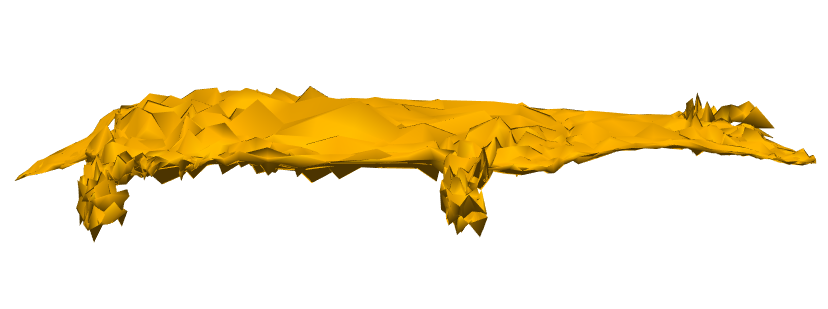
\includegraphics[width=1.0\textwidth]{figure/Cow_opt_20.png}
	\caption{sampling rate = $20\%$时OPTSPACE + CMDS恢复坐标结果的侧面图}
 	\label{fig:cow_opt_20}
\end{figure}

造成这样的原因可能就是前面所说的,前两个奇异值相较于之后的奇异值来说太大。事实上完整的$Cow$数据集的奇异值分别为$2.243\times10^3, 1.676\times10^3, 0.349\times10^3, 0.130\times10^3, 0.088\times10^3$,可以明显的发现前两个奇异值与后面三个之间的差值。同时,在前两个奇异值之间我们也能看到很明显的区别。这就验证了我们之前所说的OPTSPACE算法在矩阵条件数较大的时候效果不佳。而Incremental \\
OPTSPACE + CMDS方法相对于OPTSPACE算法来说有很大的改进。在此说明一下在应用Incremental OPTSPACE算法的过程中会发现即使每一次只计算最大的奇异值仍然不能保证有较好的效果,因此想到通过改变trimming过程和步长初值$tau$来进一步改善Incremental OPTSPACE。表\ref{tab:COW}中展示的结果为sampling rate分别为$2\%, 3\%, 5\%, 10\%, 20\%$时,trimming过程为将degree大于$1, 1, 0.8, 0.7, 0.7$倍的矩阵degree均值的行列置为零,初始步长$tau$设为$10^{-2}, 10^{-2}, 10^{-2}, 10^{-1}, 10^{-1}$时的结果。这样改变trimming过程的想法是希望在初次进行奇异值分解的时候能削弱degree较大的行与列,即较大的奇异值所产生的影响。在这样的操作之后,Incremental OPTSPACE算法的效果在原有基础上有了进一步的改善。


\begin{table}[!htbp]
\caption{SMACOF\ SVT+CMDS\ OPTSPACE+CMDS三种算法在恢复$S^2$数据集收敛或达到迭代次数上限所用时间}
\label{tab:SPHERE_TIME}
\centering
\begin{tabular}{|c|ccccc|}
\hline
\diagbox{Algorithm}{Time(s)}{Sampling rate}&$2\%$ &$3\%$ &$5\%$ &$10\%$ &$20\%$\\
\hline
\text{SMACOF} &394.3920 &120.7250 &68.6260 &90.1370 &40.6080 \\
\hline
\text{SVT + CMDS} &4246.1 &112.7820 &43.1310 &23.3750 &32.0340\\
\hline
\text{OPTSPACE + CMDS}&327.7620 &277.9470 &84.3620 &29.0830 &12.4380\\
\hline
\end{tabular}
\end{table}

\begin{table}[!htbp]
\caption{SMACOF\ SVT+CMDS\ OPTSPACE+CMDS三种算法在恢复$Cow$数据集收敛或达到迭代次数上限所用时间}
\label{tab:COW_TIME}
\centering
\begin{tabular}{|c|ccccc|}
\hline
\diagbox{Algorithm}{Time($10^3$s)}{Sampling rate}&$2\%$ &$3\%$ &$5\%$ &$10\%$ &$20\%$\\
\hline
\text{SMACOF} &4.7887 &4.7026 &2.1574 &2.0956 &2.5769 \\
\hline
\text{SVT + CMDS} &2.8380 &2.6550 &1.9729 &1.6608 &1.3542\\
\hline
\text{OPTSPACE + CMDS}&1.0910 &2.6439 &1.0924 &1.2613 &1.2763\\
\hline
\end{tabular}
\end{table}


\begin{figure}[h]
	\centering
	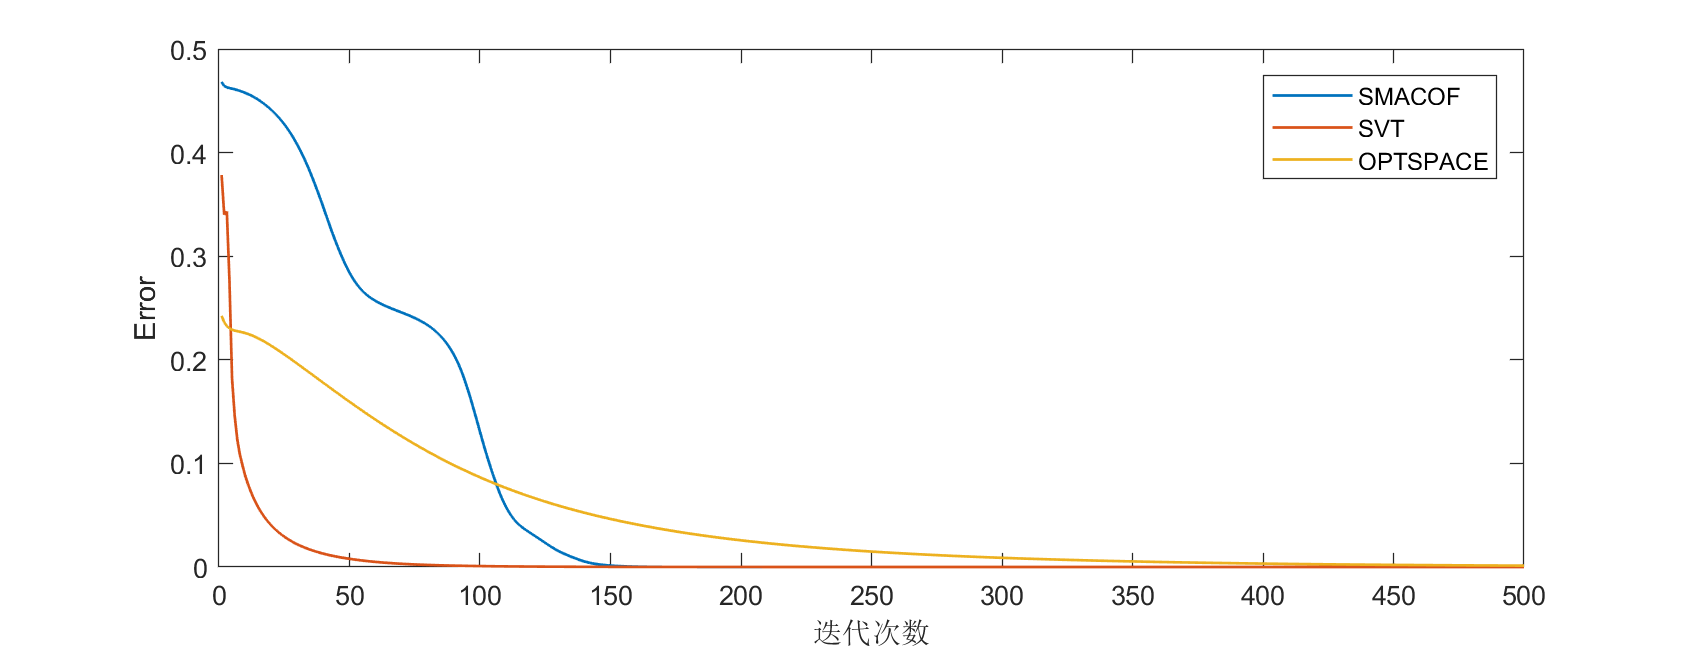
\includegraphics[width=1.0\textwidth]{figure/SphereError.png}
	\caption{sampling rate = $20\%$时三种算法恢复$S^2$数据集时Error随迭代次数变化曲线}
 	\label{fig:sphere_error}
\end{figure}


\begin{figure}[h]
	\centering
	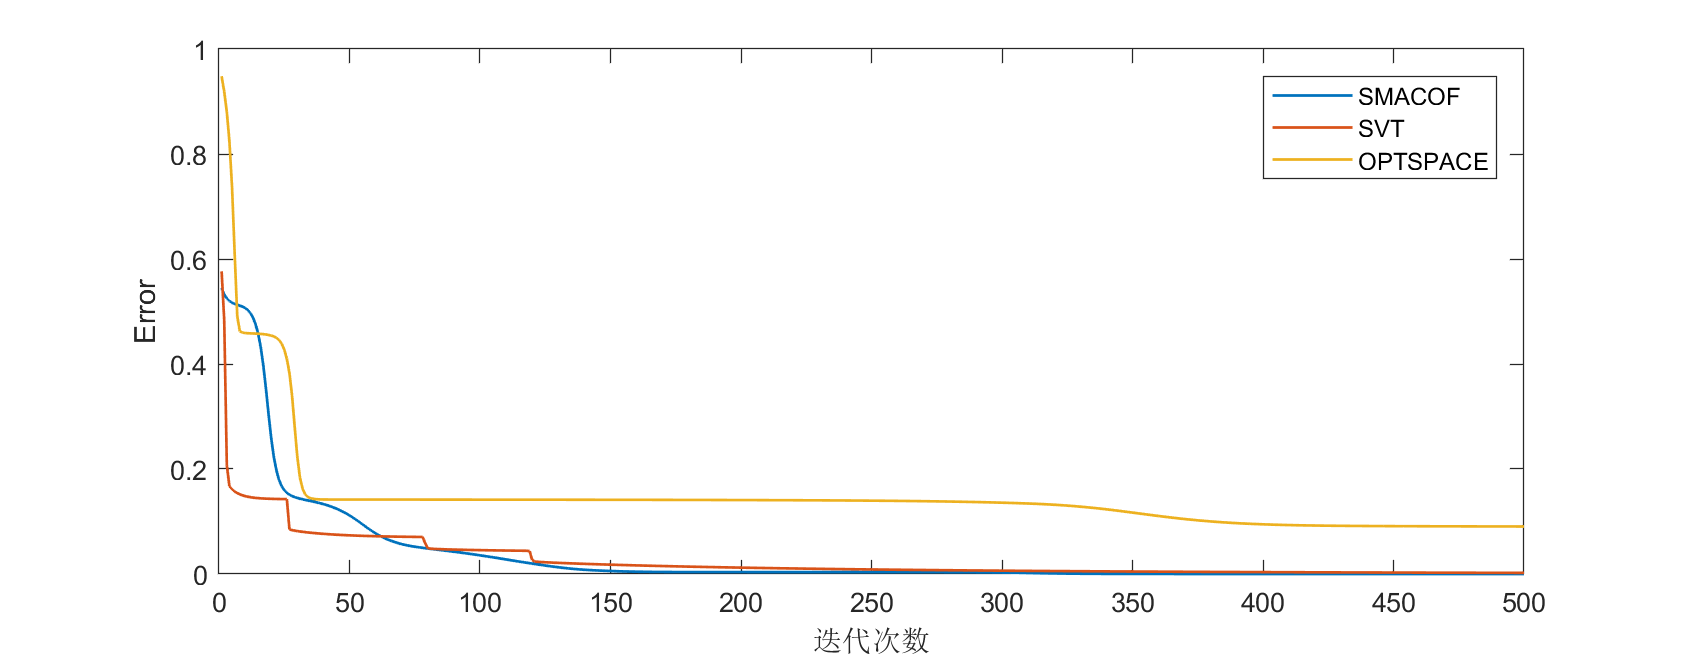
\includegraphics[width=1.0\textwidth]{figure/CowError.png}
	\caption{sampling rate = $20\%$时三种算法恢复$Cow$数据集时Error随迭代次数变化曲线}
 	\label{fig:cow_error}
\end{figure}

为进一步分析比较SMACOF, SVT + CMDS和OPTSPACE + CMDS三种算法,在表\ref{tab:SPHERE_TIME}和表\ref{tab:COW_TIME}中列出了三种算法收敛或达到最大迭代次数(1000次)所用的时间。在图\ref{fig:sphere_error}和图\ref{fig:cow_error}中展现了三种算法在两个数据集sampling rate为20的情况下,500次迭代内,Error随迭代次数的变化曲线。由于Incremental OPTSPACE + CMDS相对于其余三种算法来说多了一层对秩的循环,故不在此一起讨论。

首先,由表\ref{tab:SPHERE_TIME}和图\ref{fig:sphere_error}可以看出对于对于sampling rate为$20\%$下的$S^2$数据集,SMACOF和SVT + CMDS两个算法收敛速度很快,在前150次迭代内就可以将Error控制在一个很小的范围内。而OPTSPACE + CMDS相对于SMACOF + CMDS和SVT + CMDS而言,收敛曲线相对平缓,但却在整体用时上有明显的优势。由此可见OPTSPACE + CMDS在单次迭代过程中的运算速度很快。针对于整体其他sampling rate下的情况可以看出,SVT + CMDS算法可以在相对较短的时间和迭代次数内达到较为理想的精确度。同时如果更进一步的,在实验中使用稀疏矩阵的方式存储矩阵序列中的$\{\mathbf{Y}^k\}$,可以进一步提升运算速度。在$Cow$数据集中我们也可以得到类似的结论。由图\ref{fig:cow_error}中可以看出,和图\ref{fig:sphere_error}中一样,SMACOF + CMDS和SVT + CMDS也在200次的迭代内,误差很快就收敛到了相对较小的值,而OPTSPACE + CMDS在500次迭代之后仍保持着接近0.1的误差。这与我们之前直接对于恢复结果进行观察所得到的结论一致。在图\ref{fig:cow_error}中也可以看出OPTSPACE + CMDS算法在恢复$Cow$数据集中所存在的问题。由前面的算法描述可知,SVT + CMDS和OPTPACE + CMDS两种算法本质上都是基于奇异值分解。在SVT + CMDS算法的Error变化曲线中,我们可以清晰的看到四次阶梯型的下降变化,可以将他们分别对应到完整$Cow$数据集的5个非零奇异值。而OPTSPACE + CMDS算法的Error变化曲线中,在途中所示的500次迭代中仅展现出了三次的阶梯型下降。前两次下降的幅度很大,而最后一次的下降幅度很长的小,并且接下来曲线的变化幅度也十分的小。这也从另一个角度说明了OPTSPACE + CMDS算法在恢复$Cow$数据集时失效的原因是由于数据集的条件数过大,而不能有效的考虑那些较小奇异值和奇异向量所产生的影响。




最后,由上述数值实验的结果可以看出SMACOF算法在两个数据集下都有着相对较好的效果,而与此同时SMACOF还有一个优点,就是除了终止迭代条件和最大迭代次数之外,没有需要预先确定的参数。这使得当用于不同数据集的时候都相对方便。而SVT中的$\delta$还有OPTSPACE算法中的$\tau$需要根据经验来确定。同样在Incremental OPTSPACE中参数$\tau$还有trimming过程也涉及会影响效果的参数。例若将Incremental OPTSPACE算法中若将trimming更改成将行列degree大于1.5倍行列平均degree的置为零,同时将$\tau = 0.1$带入算法中,对于sampling rate为$1\%$的$Cow$数据集也可以达到Error也可以达到$4.991\times10^{-4}$的精确度。
        \newpage
        % 结语

    % 附录部分
    \backmatter
        % 参考文献. 因不需要纳入章节目录, 故放入附录部分
        % 实际上参考文献是属于论文主体部分
        \makereferences

        %%
% 致谢
% 谢辞应以简短的文字对课题研究与论文撰写过程中曾直接给予帮助的人员(例如指导教师、答疑教师及其他人员)表示对自己的谢意,这不仅是一种礼貌,也是对他人劳动的尊重,是治学者应当遵循的学术规范。内容限一页。
% modifier: 黄俊杰
% update date: 2017-04-15
%%

\chapter{致谢}
    首先,感谢我的指导老师李嘉教授,在大四上学期有幸上了老师的数学实验与软件一课,在课程中我掌握了MATLAB的使用技能,除此之外我还锻炼了独立思考分析问题的能力。这无论是在我课题学习和论文撰写的过程中,还是后面的学习生活中都给我了很大的帮助。由于之前没有学术研究和撰写论文的经验,在完成论文的过程中,老师不仅在大方向上给予我指导,在一些细节上的我不能理解的难点也给了我充分的提点与帮助。同时,在完成论文的过程中,由于个人事务,前期在时间安排上出现了问题。老师也耐心检查我的工作完成情况,确保论文最后的顺利完成。李嘉老师严谨的研究态度,辛勤的工作方式和有条理的对工作安排的能力是我未来工作学习的榜样,在此向李老师致以崇高的敬意和衷心的感谢。
    
    同时,感谢四年本科学习生活中学校和学院的培养。四年的本科学习中,我学到了很多的知识与技能,锻炼了独立分析问题和解决问题的能力。我相信无论我以后处于哪一个领域,从事哪一种工作,都将给予我很大的帮助。在此对所有老师的指导,教诲,还有同学们的帮助表示最诚挚的谢意。
    
	最后,要感谢我的家人,作为我最有力的精神支柱,正是他们无私的奉献和支持,让我能全心全意的投入学习和个人发展之中,让我有拼搏向前的勇气与力量。

\vskip 108pt
\begin{flushright}
	熊锦欣\makebox[1cm]{} \\
\today
\end{flushright}

    % 致谢
        \newclearpage
        % 附录
    %\appendix
    %    \include{docs/appendix1}
    %    \newclearpage
    
    
    \makeGrade      % 成绩评定记录表
\end{document}

